\ProvidesFile{the_matrix_game}[The Matrix Game]
    
\newpage

\section*{The Matrix: Game Rules}

Objective. Teams compete to correctly solve as many problems as possible from a $4\times 4$ matrix and score the highest total.

Game board. The board is a $4\times 4$ matrix of problems. Each cell is labeled by a topic and has an associated point value.

Turn order. Teams move in alternating turns.
\begin{enumerate}
\item On its turn, a team selects one unsolved cell (choosing both topic and point value).
\item The problem is shown on the screen. The team has a limited time to solve it (as set by the host).
\item When time expires, or earlier if the team declares readiness, one team member is chosen uniformly at random to present the answer on behalf of the team.
\item Scoring on the first attempt:
    \begin{itemize}
    \item If the answer is correct, the team earns the full point value of the cell.
    \item If the answer is incorrect and the opposing team is ready to answer, the opposing team may immediately attempt an answer in the same turn (without additional preparation). A random member of that team presents the answer. If correct, the opposing team earns the full point value.
    \item If the opposing team also answers incorrectly, the problem is removed from play (it “burns”).
    \item If the opposing team declines to answer, the problem remains on the board but its point value is halved for future attempts.
    \end{itemize}
\item After the resolution of the current cell, the turn passes to the other team.
\end{enumerate}

Bonuses. A team receives a bonus of 10 points for each row and for each column in which that team has correctly solved all problems.

End of the game. The game ends when the time expires or when all problems have been resolved. The winner is the team with the greater total score.

\bigskip
\begin{center}
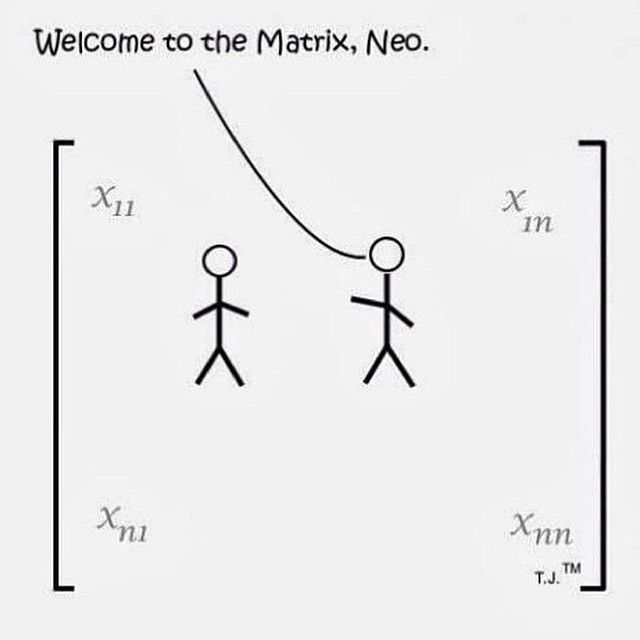
\includegraphics[scale=0.4]{Images/neo.jpg}
\end{center}

\newpage
Determinant, 10
 
    Given square matrices $A$ and $B$ of size $2025 \times 2025$ such that $\det(A) = 2$ and $\det(B) = 25$. Find $\det(BA)$.
   


\newpage

Determinant, 20
 
    Find the determinant of the following $10 \times 10$ matrix:
    $$
    \begin{pmatrix}
        10 & 0 & 0 & \dots & 0 \\
        9 & 10 & 0 & \dots & 0 \\
        8 & 9 & 10 & \dots & 0 \\
        \vdots & \vdots & \vdots & \ddots & \vdots \\
        1 & 2 & 3 & \dots & 10 \\
    \end{pmatrix}.
    $$
    


    \newpage
Determinant, 30
 
        Let $A$ be a square $2 \times 2$ matrix with $\det(A) = 2$, $B$ be a square $5 \times 5$ matrix with $\det(B) = 5$, $C$ be a rectangular $2 \times 5$ matrix and $O$ be a zero matrix of size $5 \times 2$.
        Find 
        $$
        \det\begin{pmatrix}
            A & C \\
            O & B \\
        \end{pmatrix}.
        $$
        


\newpage
Determinant, 40

    % answer: -8
    
        Find the determinant of the following matrix:
    $$
    \begin{pmatrix}
        1 & 2 & 3 \\
        5 & 1 & 4 \\
        3 & 2 & 5 \\
    \end{pmatrix}.
    $$
    


\newpage
Rank and dimension, 10
 
    Find the rank of the matrix:
   $$
   A =\begin{pmatrix}
       1 & 1 & 3 & 4 & 5 \\
       0 & 0 & -1 & 2 & -1 \\
       0 & 0 & 0 & 14 & 15 \\
       0 & 0 & 0 & 28 & 30 \\
   \end{pmatrix}.
   $$
   

   \newpage   
Rank and dimension, 20


 
    Find the dimension of the solution space of the homogeneous system $A x = 0$ with matrix:
   $$
   A =\begin{pmatrix}
   1 & 1 & 0 & 4 & 5 \\
   0 & 2 & 5 & 2 & -1 \\
   0 & 0 & 0 & 14 & 15 \\
\end{pmatrix}.
   $$
 

 \newpage
Rank and dimension, 30

 
    Does the set of all $5 \times 5$ matrices with real entries and zero trace ($a_{11} + a_{22} + a_{33} + a_{44} + a_{55} = 0$) form a vector space? If yes, find a basis and the dimension of this vector space. If no, explain why.
    

\newpage
Rank and dimension, 40

    % 35.11 а Кострикин
    
        Find a basis and the dimension of the linear span of the following system of vectors:
    $$a_1=(1,0,0,-1), \quad a_2=(2,1,1,0), \quad a_3=(1,1,1,1), \quad a_4=(1,2,3,4), \quad a_5=(0,1,2,3).$$
    

\newpage
Vector space, 10

    Consider the vector space of all polynomials of degree at most $7$ with real coefficients:
    $$
    S = \{a_0 + a_1 x + a_2 x^2 + \cdots + a_7 x^7 \mid a_i \in \R\}.
    $$
    Find a basis and the dimension of this vector space.
    

    \newpage
Vector space, 20


    
    Consider a set of all continuous functions on the interval $[0, 1]$, such that $f(x) \neq 0$ for all $x \in [0, 1]$. Is this set a vector space? If yes, find a basis and the dimension of this vector space. If no, explain why.
    
    
\newpage
Vector space, 30


    %34.14 а Кострикин
    
    Prove that the given system of vectors is linearly independent, and complete it to a basis of the space of rows:
    $$a_1=(2,2,7,-1), \quad a_2=(3,-1,2,4), \quad a_3=(1,1,3,1).$$   
     

\newpage
Vector space, 40

    %34.10 б) Кострикин
    
    Let the vectors $e_1, e_2, e_3$ and $x$ be given by their coordinates in some basis:
    $$e_1=(2,1,-3), \quad e_2=(3,2,-5), \quad e_3=(1,-1,1), \quad x=(6,2,-7).$$
    Prove that $(e_1, e_2, e_3)$ is also a basis of the space, and find the coordinates of $x$ in this basis. 

    

\newpage
Yet another matrix, 10

 
    Given a square matrix $A$ of size $2025 \times 2025$ with $\det(A) = 25$. Find $\det(A^{-1})$.
   

   \newpage
Yet another matrix, 20


   
    Find the inverse of the following matrix:
$$
\begin{pmatrix}
    1 & 2 & 0 & 0 & 0 & 0 \\
    0 & 1 & 0 & 0 & 0 & 0 \\
    0 & 0 & 0 & 1 & 0 & 0 \\
    0 & 0 & 1 & 0 & 0 & 0 \\
    0 & 0 & 0 & 0 & 5 & 0 \\
    0 & 0 & 0 & 0 & 0 & 10
\end{pmatrix}.
$$
 

\newpage
Yet another matrix, 30

 
Does the set of all invertible $5 \times 5$ matrices with real entries form a vector space? If yes, find a basis and the dimension of this vector space. If no, explain why.
 

\newpage
Yet another matrix, 40

    %34.11 a) Кострикин
    
        Prove that each of the two given systems of vectors $S$ and $S^{\prime}$ is a basis. Find the transition matrix $C$ from $S$ to $S^{\prime}$ ($e^{\prime} = e C$):
        $$
        \begin{aligned}
        & S=((3, 1, 0),(2, 1, 0),(2, 3, 1)) \\
        & S^{\prime}=((1, 2, 1),(2, 3, 3),(3, 8, 2))
        \end{aligned}
        $$
